\chapter{Three Tricks in Training of Neural Network}

\section{Reviewing}
\begin{itemize}
\item
Why Kaiming initialization is not good enough for deep narrow network (i.e., large $L/d$)?

Answer:
Error accumulation, i.e.,
\[
\text{error}\sim\exp(L/d)
\]
\item
Besides random initialization, what else is possible?

Answer: 
orthogonalization.
\item
Besides weight matrices $ W^{1:L}$, what eles can be tuned at initialization?

Answer: 
Input strength~(size) $\|x\|^2$.
\end{itemize}

\paragraph{Motivation}
Up to today, there are three tricks to train a deep neural network:
\begin{enumerate}
\item
Intialization;
\item
Batch Normalization;
\item
Residual units (architecture)
\end{enumerate}
Back to 2012, there were  $6$-$10$ tricks to train the AlexNet. As time goes by, scientists found that many of these tricks are not necessary.
In this lecture, we will talk about highlights in these three tricks.

\section{Intialization: Dynamical Isometry}
Up to now, Dynamical Isometry is the peak of initilization theory for deep learning.
Given a neural network $\text{NN}:\mathcal{X}\to\mathcal{Y}$ such that
\[
y = \text{NN}(x;W),
\]
the goal is to choose $W$ such that $\|y\|\approx \|x\|,\forall x$. More precisely, we want to make singular values of the input-output Jacobian $J$ all close to $1$.
Following the notation setting in section~(\ref{sec:1:3}), we have
\[
J=\frac{\partial z^L}{\partial z^0} = \prod_{\ell=1}^L\frac{\partial z^{\ell}}{\partial z^{\ell-1}} = \prod_{\ell=1}^L(D^{\ell}W^{\ell})
\]
with $D^{\ell} = \diag(\phi'(\{h_i^{\ell}\}_{i=1}^{d_{\ell_i}}))$.

The key turns to the understanding of the distribution of eigenvalues of the matrix $JJ\trans$ (i.e., singular values of $J$).
There is a classical theory for the eigenvalues of random matrix, which claims that its distribution is like a semi-circle:
\begin{figure}[H]
\centering
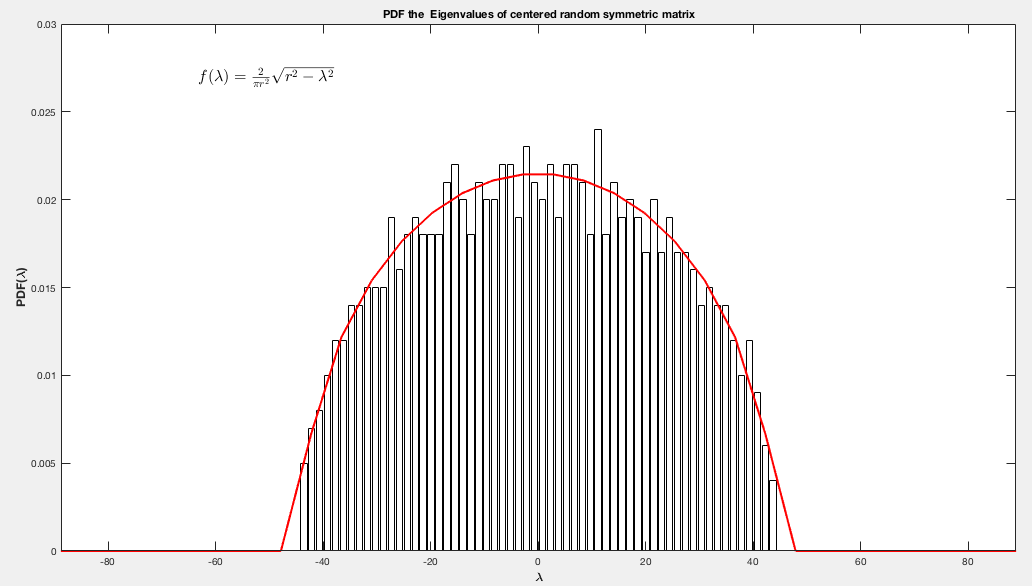
\includegraphics[height=0.4\textwidth]{Forth_lecture/f_3}
\caption{
The pdf of eigenvalues for the scaled (symmetric) random matrix $\frac{1}{\sqrt{N}}W$ with $N=1000$ and $w_{i,j}$ follows normal distribution.{The simulation code is in 
{{https://www.mathworks.com/matlabcentral/fileexchange/46464-wigner-s-semicircle-law}}}
}
\end{figure}
\begin{theorem}[Wigner's semi-circle law]
Given a symmetric matrix $W\in\mathbb{R}^{N\times N}$ whose entries $W_{i,j},i\ge j$ are independent random variables, the asymptotic distribution~(as $N\to\infty$) of the eigenvalues of $W$ is like a semi-circle.
\end{theorem}

The semi-circle law is related to our problem:
The Jacobian $J$ is a random matrix, 
This semi-circle law is related to our problemm where the randomness comes from $W$.
More precisely, it is a product of nonlinear function of random matrices.
In order to resolve the nonlinearity, we need to use the free probability(i.e., $S$-transform) tool to calculate the distribution of singular values of $J$.

\paragraph{The possibility of dynamical isometry}
The paper (\cite{DBLP}) gives possibility for realizing dynamical isometry for deep \emph{nonlinear} neural networks in different scenarios.
\begin{table}[H]
  \centering
    \caption{Summarization of the results for the possibilities for realizing dynamical isometry for deep neural networks with different types of activations and initializations}
  \label{tab:1}
  \begin{tabular}{ccc}
    \toprule
    &  Scenarios & possibilities\\
    \midrule
    Section~(2.5.1)  & \tabincell{c}{Guassian Initialization\\ +Relu Activation} & No \\\hline

    Section~(2.5.1)  & \tabincell{c}{Guassian Initialization\\ +Hard-tanh Activation} & No \\\hline
    Section~(2.5.2)  & \tabincell{c}{Orthogonal Initialization\\ +Relu Activation} & No \\\hline
    Section~(2.5.2)  & \tabincell{c}{Orthogonal Initialization\\ +Hard-tanh Activation} & Yes \\
    \bottomrule
  \end{tabular}
\end{table}
In particular, for the last scenario, one can achieve dynamical isometry by tuning $\|x\|^2,\sigma_w^2,\sigma_b^2$ properly\footnote{Here $\sigma_w^2\triangleq\frac{1}{d}\text{var}(w_{i,j}^{\ell})$ and $\sigma_b^2$ refers to the variance of bias for pre-activation}. In this case, the deep neural network enjoys depth-independent training time.

The mechanism for dynamical isometry is to realize three goals simultaneously, i.e., relies on solving three types of equations:
\begin{itemize}
\item
Feedforward propagation: keep variance
\item
Backforward propagation: keep variance
\item
Eigenvalues of $J\trans J$ close to $1$.
\end{itemize}
The realization relies on choosing $\|x\|^2,\sigma_w^2,\sigma_b^2$. The failure of first three scenarios in Table~(\ref{tab:1}) is due to the loss of freedom of these variables.

\paragraph{Why ``Orthogonal'' is ``Difficult''}
Before the paper (\cite{pmlr-v80-xiao18a}) comes out, the orthogonal initialization for CNN is difficult, One reason is that the orthogonality for this architecture is not well-defined:
\begin{itemize}
\item
For fully connected neural network, we say the weight matrix is orthogonal if $W\trans W=I$.
\item
For CNN, consider the pre-activation process, i.e., $y=W\otimes x$, it is unclear how to define the orthogonality for tensor product.
To resolve this issue, the paper (\cite{pmlr-v80-xiao18a}) defines the orthogonality as $\|y\|=\|x\|,\forall x$.
\end{itemize}
After designing the orthogonal weights for CNN, they are able to train 10000-layer-net for CIFAR10.
This result indicates that initialization is enough for training ultra-deep neural network.

\section{Batch Normalization}
\paragraph{Motivation}
Previous data analysis knowledage tells us that the success of data processing also depends on the \emph{input normalization}~(pre-processing of data), even for linear regression.
It's nature to do the similar thing for the training of neural networks.
\begin{example}
Review the linear regression problem.
Given the data points $(x_i,y_i)$ for $i=1,\dots,n$, one wants to select parameter $w^*$ such that the quadratic loss is minimized:
\[
w^*=\arg\min_{w\in\mathbb{R}^d}\frac{1}{n}\sum_{i=1}^n(w\trans x_i - y_i)^2
\]
For the data matrix $X=[x_1,x_2,\dots,x_n]$, one should always do the row normalization:
\[
\begin{bmatrix}
x_1&x_2&\cdots&x_n
\end{bmatrix}\xrightarrow{\eta}
\begin{bmatrix}
\tilde{x}_1&\tilde{x}_2&\cdots&\tilde{x}_n
\end{bmatrix}
\]
where $\tilde{x}_i\triangleq\frac{x_i - \mu}{\sigma}$ with $\mu=\left[\frac{1}{n}\sum_ix_{i,j}\right]_j$ and $\sigma=\left[1/n\cdot\sum_i(a_{i,j}-\mu)^2\right]_j$. Here the minus and division operator is performed \emph{component-wisely}.

From the perspective of optimization, this opertion improves the \emph{convergence speed}, since the operator $\eta$ will reduce the condition number\footnote{
$\kappa(X)=\lambda_{\max}(X)/\lambda_{\min}(X)$ denotes the condition number of $X$, see Prof. Luo's Note Lecture 2 for more detailed explanations.
} of the data matrix.

From the experience of linear regression, we gain some knowledge for the training of neural nets:
\begin{itemize}
\item
It is necessary to do pre-processing of the input.
\item
Besides, for each layer, we might have the same issue that the condition number for variables before activation is large or small.
\end{itemize} 
Before (\cite{Glorot10understandingthe}), people uses the layerwise-per training technique, which also brings up some problems such as the inefficiency of training.
Therefore, we need other techniques to solve the issue.

Consider the neural network represented in the figure below:
\begin{center}
\smartdiagramset{back arrow disabled=true,
text width=1.5cm
}
\smartdiagram[flow diagram:horizontal]{
$[x(1:n)]$,
$[z^1(1:n)]$,
$[z^2(1:n)]$,
$\cdots$
}
\end{center}
where $z^{\ell}$'s are variables before activation. 
The goal is to make matrices 
\[Z^{\ell}=
\begin{pmatrix}
z^{\ell}(1)&\cdots&z_1^{\ell}(n)
\end{pmatrix}=\begin{pmatrix}
z_1^{\ell}(1)&\cdots&z_1^{\ell}(n)\\
\vdots&\ddots&\vdots\\
z_d^{\ell}(1)&\cdots&z_d^{\ell}(n)\\
\end{pmatrix}
\]
 become well-conditioned for each $\ell=1,\dots,L$, i.e., each row has zero mean and unit variance.\footnote{The $i$-th row denotes the data points for the $i$-th feature, and the row normalization makes these data points well-scaled}
\end{example}

To fully understand how the batch normalization achieves the row normalization for each data matrices $Z^{\ell}$, consider the toy example presented below:

\begin{example}[Toy Example]
Consider an aritificial problem defined as
\begin{equation}\label{Eq:4:1}
\begin{array}{ll}
\min_{h}&F(h)\triangleq\sum_{i=1}^ng(h_i)\\
\mbox{with}&\sum_ih_i=0\\
&\sum_ih_i^2=1
\end{array}
\end{equation}
Combining with gradent descent method, there are at least 3 ways to deal with it:

\paragraph{Method 1: Pure Algorithmic Correction}
The intuitive way is that in each iteration one performs the gradent descent, and then project the new iterates within the constraint set. 
However, the projection into this constraint set could be diffucult due to its non-convexity. 
Therefore, we modify the projection step with the \emph{normalization operator} $\eta$:
\[
\begin{array}{ll}
\eta(h_{1:n})&\triangleq \frac{h_{1:n} - \mu}{\sigma}\\
\text{with}&\mu = \frac{1}{n}\sum_i h_{i}\\
&\sigma = \frac{1}{n}\sum_i\|h_i - \mu\|^2
\end{array}
\]
The whole algorithm is presented below:
\[
\left\{
\begin{aligned}
h^{t+1/2}&\leftarrow h - \nabla F(h)\\
h^{t+1}&\leftarrow \eta(h^{t+1/2})
\end{aligned}
\right.
\]

\paragraph{Method 2: Constrained optimization}
Consider this problem as a constrained optimization problem, and thus it's natural to solve this problem from its dual~(or solve primal and dual simultaneously), e.g., applying Lagrangian method or ADMM.

\begin{remark}
The method 1 solves the problem in an algorithmic way, i.e., modify the gradient project method in a heuristic way;
The method 2 is more about reformulation, i.e., reformulate this problem from its dual and therefore solve the new convex problem instead.
We observe that both of them don't work well in practice. The method 3 reformulates this problem in another way and we found it works well.
\end{remark}
\paragraph{Method 3: New way of Formulation}
We reformulate this problem into unconstrained optimization, by substituting the constraint into the objective function:
\begin{equation}\label{Eq:4:2}
\begin{array}{ll}
\min_h&F(\eta(h))
\end{array}
\end{equation}
Then the optimal solution of the origin problem~(\ref{Eq:3:1}) is tractable by setting $h^*=\eta(\arg\min_hF(\eta(h)))$.
For this unconstrained optimization problem, we can apply the gradient descent to solve it.
\end{example}

\paragraph{Motivation for Batch Normalization~(BN)}
The insights of BN is similar to that in Method 3. 
Consider a $2$-layer neural network computing
\begin{equation}\label{Eq:4:3}
e = F_2(F_1(x,W_1),W_2)
\end{equation}
where $F_1,F_2$ are arbitary transformations, and the parameters $W_1,W_2$ are to be chosen so as to minimize the loss $e$. 
Learning $W_2$ can be viewed as if the inputs $z\triangleq F_1(x,W_1)$ are fed into the sub-network
\[
e = F_2(z,W_2).
\]
The goal for BN is to ensure the distribution of nonlinearity inputs (i.e., $z$) remains more stable during the training process, i.e., pick $W_2,W_2$ to minimize the loss function and within the constraint set
\[
\mathbb{E}[x]=0,\text{Var}[x]=1,\qquad
\mathbb{E}[z]=0,\text{Var}[z]=1.
\]
From the experience of Method 3, it suffices to reformulate (\ref{Eq:4:3}) by adding the \emph{normalization} process before the non-linear activation in each layer.
\begin{figure}[H]
\centering
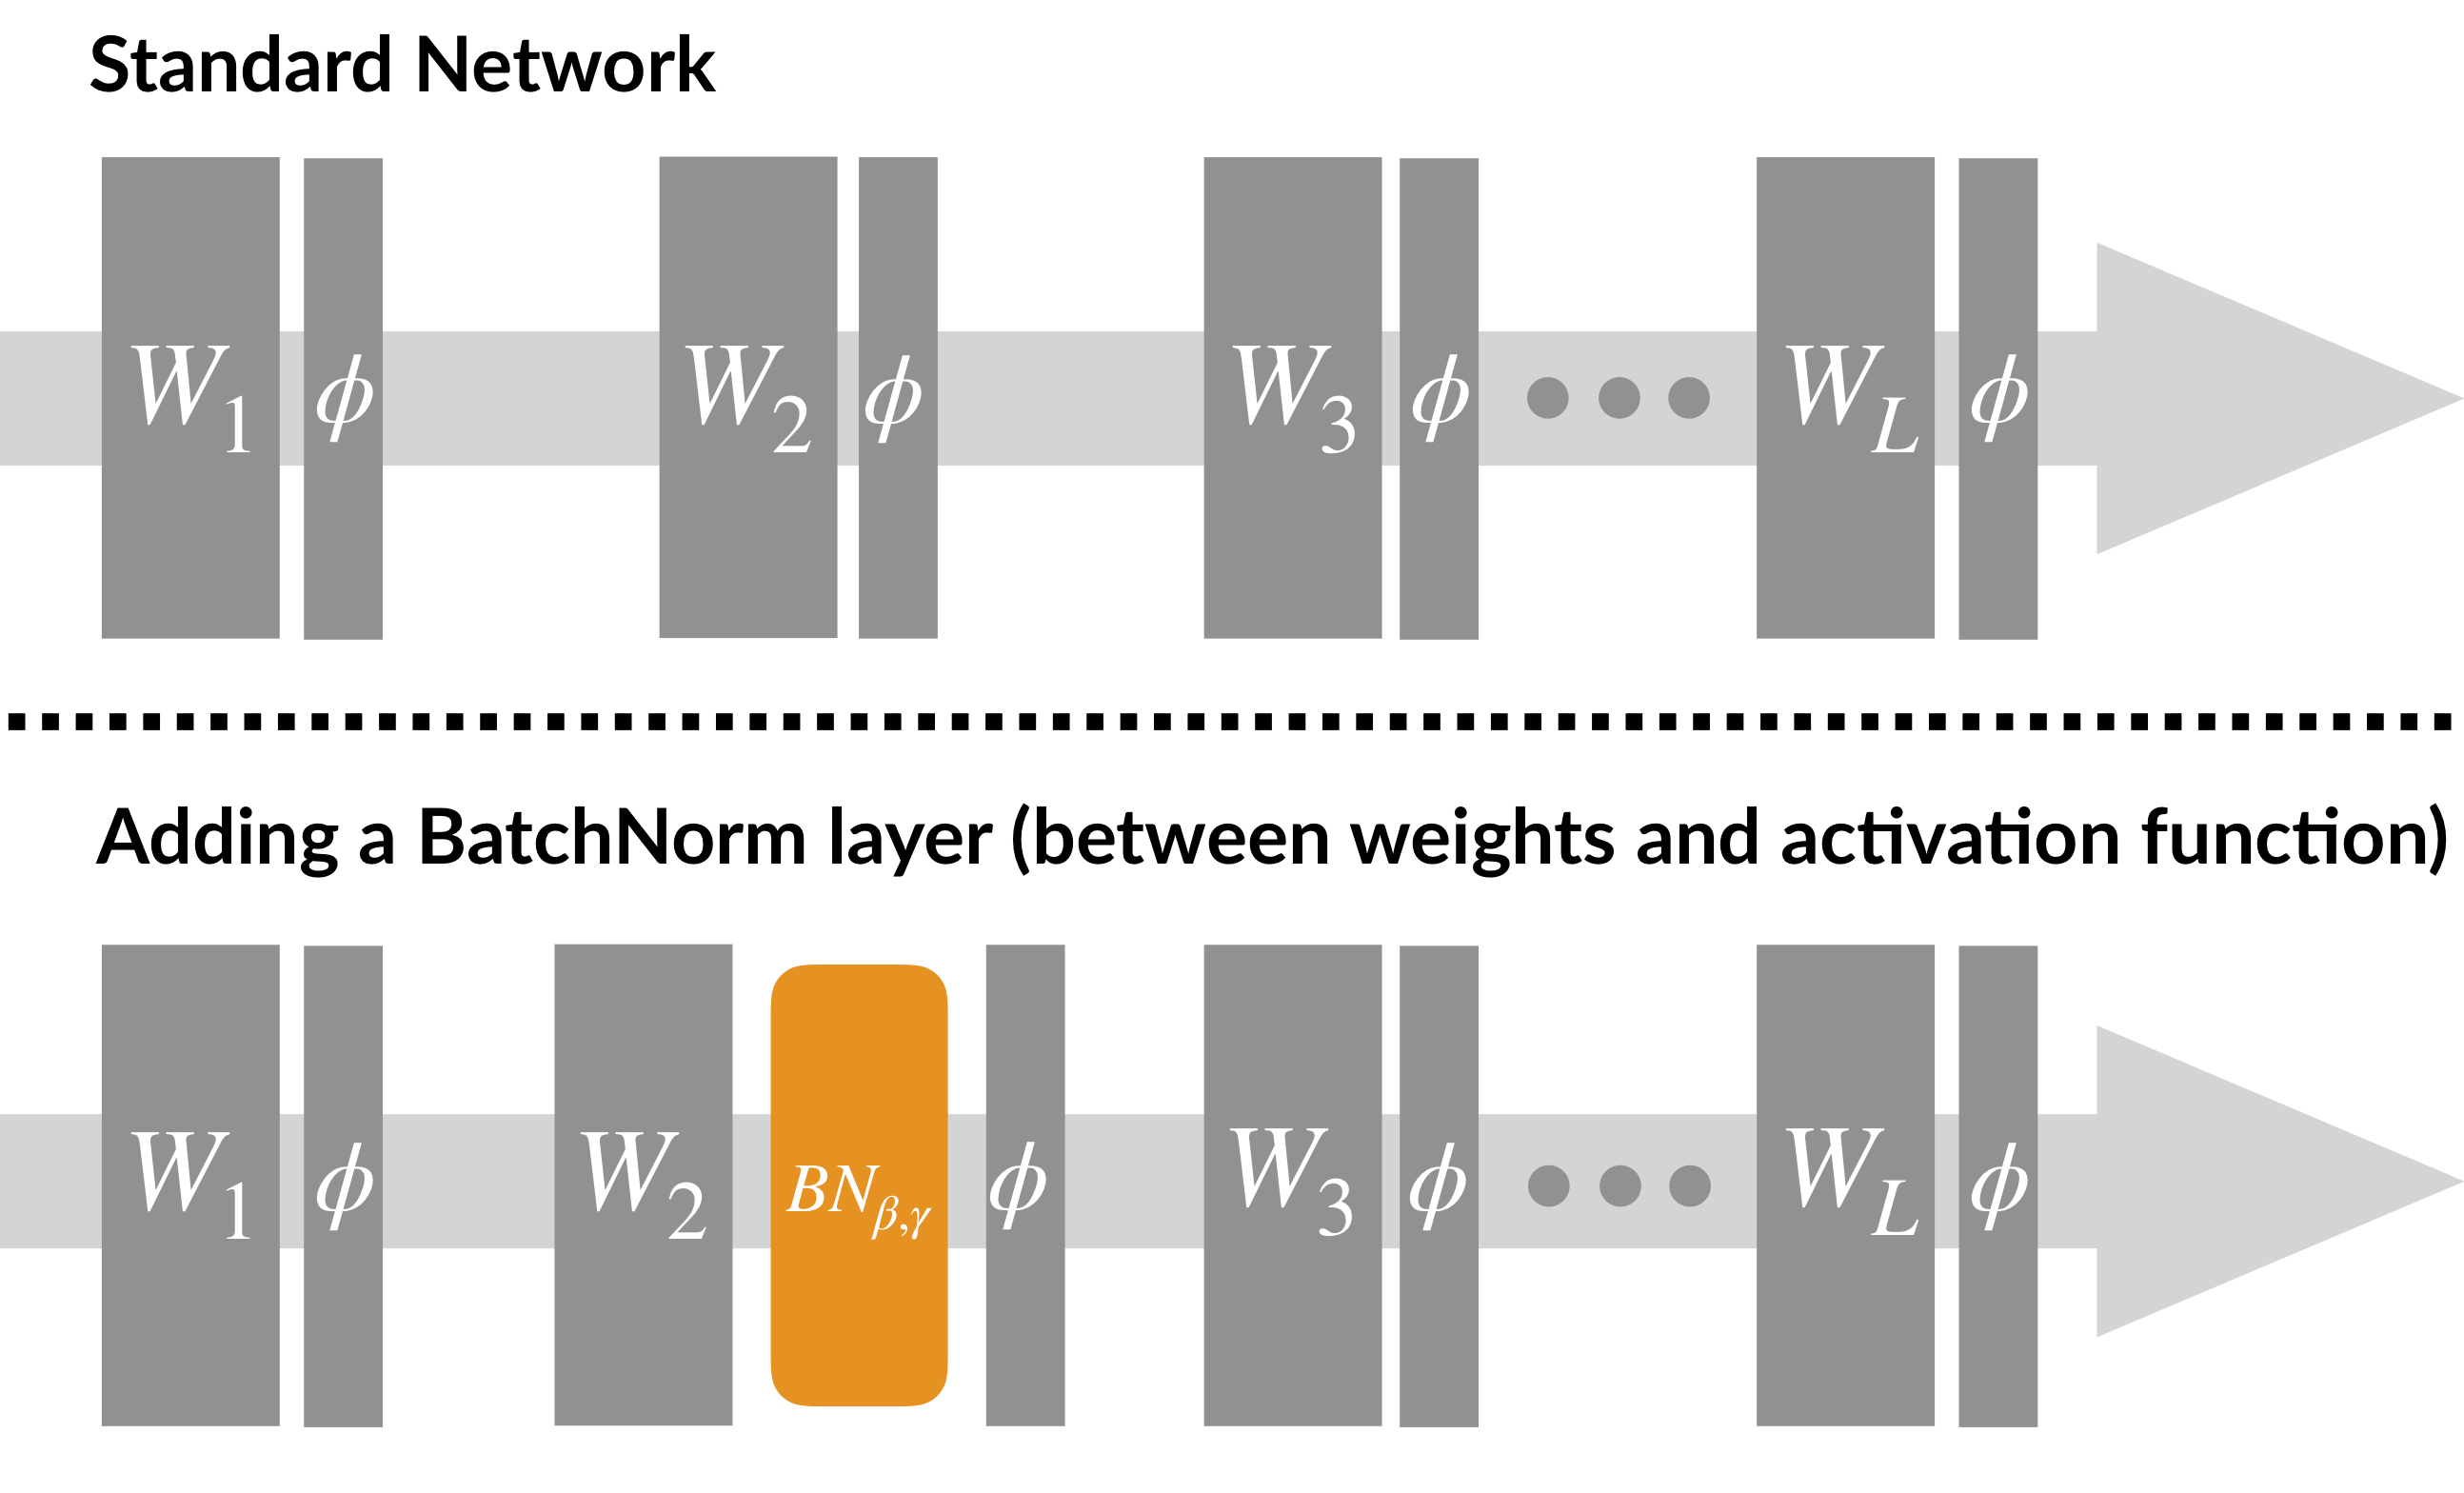
\includegraphics[width=0.7\textwidth]{Forth_lecture/f_4}
\caption{Adding the Bacth Normalization process in the \emph{second} layer}
\end{figure}
The \emph{normalization} process can be changed in different scenarios, e.g., for capsule-net, change it with the \emph{clustering} process.

\paragraph{Gradient Computation if adding the BN}
The standard one-layer neural network can be described as a non-linear parametric function
\[
z = g(Wu),
\]
where $g$ is the non-linear transformation, $W$ is the weight matrix.
By adding the BN, the standard function is replaced with
\[
z =  g(\text{BN}(Wu)),
\]
where the BN transform is applied independently to each dimension of $x=Wu$.
We set $h = Wu$, then we show how to compute $\frac{\partial z}{\partial h}$:
\begin{enumerate}
\item
Step 1: decompose the transformation from $h$ to $z$ into paths.

Note that $z = z(h,\mu(h),\sigma(h))$. Therefore, the paths could be:
\begin{align*}
h&\to z;&\quad\text{provided that $\mu,\sigma$ are fixed}\\
h&\to \mu\to z;\\
h&\to\sigma\to z.
\end{align*}
\item
Step 2: Apply the Chain Rule.
\[
\frac{\tilde{\partial} z}{\tilde{\partial} h} = 
\left.\frac{\tilde{\partial} z}{\tilde{\partial} h}\right|_{\mu,\sigma \text{ fixed}}
+
\frac{\tilde{\partial}{z}}{\tilde{\partial}\mu}\frac{\tilde{\partial}\mu}{\tilde{\partial} h}
+
\frac{\tilde{\partial}{z}}{\tilde{\partial}\sigma}\frac{\tilde{\partial}\sigma}{\tilde{\partial} h}
\]
in which the notion of generalized Jacobian is adpoted.

\end{enumerate}
\begin{remark}[Representation Power]
Re-consider the formula~(\ref{Eq:4:1}). We find that
\[
\{F(h)\mid h\in\mathbb{R}^n\}\supseteq \{F(\hat{h})\mid \sum_i\hat{h}=0,\sum_i\hat{h}^2=1\}.
\]
Therefore, the $\min F(h)$ is not necessarily equivalent to $\min F(\eta(h))$.
In order to resolve this issue, we need to ``store'' the representation power by scale and shift $\eta(h)$ in~(\ref{Eq:4:2}), i.e., introducing $\gamma,\beta$ to form a new problem
\begin{equation}\label{Eq:4:4}
\min_{h,\gamma,\beta}F(\gamma\cdot\eta(h)+\beta)
\end{equation}
Now the set $\{F(h)\mid h\in\mathbb{R}^n\}
=\{F(\gamma\cdot\eta(h)+\beta)\mid h\in\mathbb{R}^n,\gamma,\beta\in\mathbb{R}\}
$.
\end{remark}
In the remaining of this section, let's discuss more about applying BN in practice.

\begin{figure}[H]
\centering
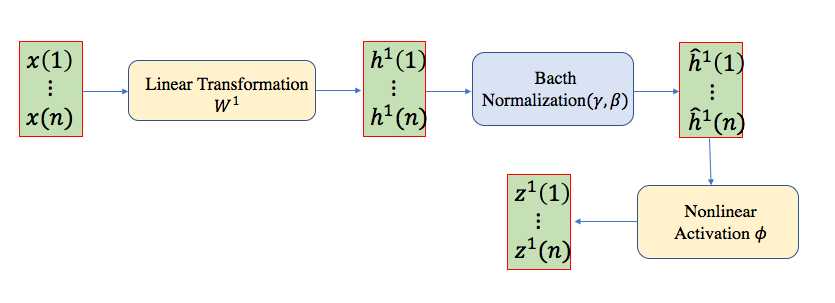
\includegraphics[width=\textwidth]{Forth_lecture/f_5}
\end{figure}
\begin{remark}
Batch Normalization is applied before the non-linear activation in each layer.
\end{remark}
\begin{remark}
The function $\text{BN}_{\gamma,\beta}(\cdot)$ is applied to each row of the matrix
\[
\begin{pmatrix}
h^1(1)&\cdots&h^1(n)
\end{pmatrix}.
\]
\end{remark}
\begin{remark}
In practice, the BN is applied for mini-batch with batch size $B$. 
In other words, the total $n$ inputs are separated into $N$ batches, where each batch contains $B$ inputs. The BN is performed on each single batch.
This technique changes the problem form:
\[
\begin{array}{ll}
\mbox{Standard Formulation}&\min_{\theta}\frac{1}{n}\sum_{i=1}^n\ell(f_\theta(x_i),y_i)\\
\mbox{Mini-Batch Formulation}&\min_{\theta}\frac{1}{N}\sum_{i=1}^N\tilde{\ell}(\tilde{f}_\theta(x_{i,1:B}),(y_{i,1:B}))
\end{array}
\]
Previously, the neural network is a single-input-single-output~(SISO) function:
\[
x_i\xrightarrow{f_{\theta}}\hat{y}_i
\]
Now, with mini-batch BN, the neural network is a multi-input-multi-output~(MIMO) function:
\[
x_{i,1:B}\xrightarrow{\tilde{f}_{\theta}}\hat{y}_{i,1:B}
\]
\end{remark}

\begin{remark}
In each batch $i$, $\tilde{f}_{\theta}$ is also dependent on the parameter $\bar{\mu}_i,\bar{\sigma}_i$. 
Therefore, for the whole neural network $\tilde{f}_{\theta}(\bar{\mu},\bar{\sigma})$, there could be an issue about how to select the parameters $\bar{\mu}$ and $\bar{\sigma}$.
\end{remark}
\begin{remark}
For the problem~(\ref{Eq:4:4}), if we choose $\gamma=\|h\|$ and $\beta=\frac{1}{n}\sum_ih_i$, then the representation power is strong, but we may have difficulty in training, i.e, solving this optimization problem;
if we choose $\gamma=1$ and $\beta=0$, it will lead to the weak representation power. Therefore, the choice of $\gamma,\beta$ is a trade-off.
\end{remark}
\begin{remark}
An reasonable mini-bacth size is needed to calculate $\mu,\sigma$ in each single bacth, i.e., $B\ge16,32,\dots$.
For non-ImageNet tasks, it will be an issue on how to choose $B$.
\end{remark}
\begin{remark}
Besides BN, there are other types of normalization methods:
\begin{itemize}
\item
Layer normalization; (which is standard in language processing)
\item
Instance normalization;
\item
Weight normalization;
\item
Group normalization; (\cite{Wu_2018_ECCV})
\item
Column normalization. The intuition is that there are lots of headache come from normalizing rows, it may be better to normalize columns instead. We skip the discussion for column normalization in this lecture.
\end{itemize}
\end{remark}



\section{ResNet}
Recommended Reading: (\cite{He2016res}).
\paragraph{Motivation}
It is intuitive that more layers for neural networks will lead smaller traning error. However, some numerical experiments show it is not true in general:
\begin{figure}[H]
\centering
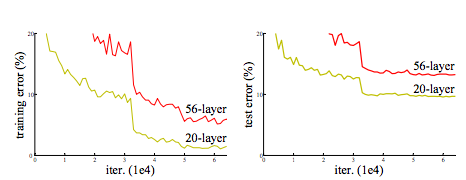
\includegraphics[width=0.7\textwidth]{Forth_lecture/f_7}
\caption{
Training error~(left) and test error~(right) on CIFAR-$10$
with $20$-layer and $56$-layer ``plain'' networks. The deeper network
has higher training error, and thus test error. Similar phenomena
on ImageNet is also observed.
}
\label{fig:4:3}
\end{figure}
Let's analysis what is the most possible reason leading to this phenomena.
Let's introduce few terminologies first.
In data science, the testing error can be separated into three types of errors:
\begin{itemize}
\item
Representation Error, which is related to the representation power of the fitting model.
\item
Optimziation Error, which is related to how well we minimize the loss function.
\item
Generalization Error, which is related to the over-fitting issue.
\end{itemize}
In Fig.~\ref{fig:4:3} we observe that the training error for $56$-layer network is larger. There are two factors related to the training error:
\[
\mbox{Tranining error}=\left\{
\begin{aligned}
\mbox{Representation Error}+\\
\mbox{Optimziation Error}
\end{aligned}
\right.
\]
It seems that the high training error for deeper neural network is because of the optimziation error, since deeper neural network admits stronger power in representation.

The optimization error for solving $\min_{\theta}F(\theta)$ using iteration formula can also be decomposed into two types of errors:
\[
\underbrace{[F(\hat{\theta}) - F^*]}_{\text{Optimization Error}} = 
\underbrace{[F(\hat{\theta}) - F(\theta^\infty)]}_{\text{Convergence Error}} 
+ 
\underbrace{[F(\theta^\infty)  - F^*]}_{\text{Global-optimality Gap}}
\]
Here $\theta^\infty$ is the solution we can obtain if given $\infty$ many iterations, i.e., the limit point where the optimiztion algorithm converge to.
\begin{itemize}
\item
If $F(\theta^\infty) - F^*$ is large, one often needs reformulation of the original problem and smart initialization.~ Check (\cite{frankle2018the}) with its comments (\cite{WinNT}) in Zhihu.
\item
If $F(\hat{\theta}) - F(\theta^\infty) $ is large, one often improves his algorithm to accelerate, such as momentum-based acceleration.
\end{itemize}

It seems that the global-optimality gap is large for our training, and therefore some smart initialization is needed.
Moreover, one may ask does $56$-layer have more ``representation power'' than $20$-layer networks?
Not neceesarily, unless the extra $36$-layer can be approximated to the identity operator.

It's known that the deep neural network is sensitivity to initialization, i.e., we can only travel a small region around the initialization.
Therefore, it seems that the high training error for deep neural network is because that we may never travel have chance to travel to the identity operator for the extra $36$-layer operations.


\paragraph{Solution}
The solution for solving this issue is to design the architecture to recover the identity operator. The Resnet is designed:
\[
f_{\theta}(x) = \mathcal{F}(x,\{W_i\})+x,
\]
where $x$ is the input vectors of the layers.
More generally, for same-width network in the layer $\ell=1,\dots,L$,
\[
z^{\ell} = \phi(W^{\ell}z^{\ell-1}) + z^{\ell-1},\quad
\]

\begin{remark}
The dimension of input and output does not always match. Two tricks may be needed:
\begin{itemize}
\item
Perform a linear projection $W_s$ by the
shortcut connections to match the dimensions:
\[
f_{\theta}(x) =\mathcal{F}(x,\{W_i\})+W_sx.
\]
\item
Use pooling to change the dimension.
\end{itemize}
\end{remark}

\begin{remark}
ResNet uses $2$-layer and $3$-layer net as residual module.
\end{remark}

\begin{remark}
Motivated by LSTM, the paper~(\cite{srivastava2015highway}) uses ``gate'' to resolve this issue, but their performance is no better than ResNet.
\end{remark}









